\ifx\allfiles\undefined
\documentclass{XDBAthesis}
\def\pictures{}
\begin{document}
\else
\fi
\chapter{关键技术}
本章将介绍本算法中的几个关键技术。


%\section{架构设计}
%
%    在已经搭建好了编译环境后,接下来主要进行两部分的开发:首先主要是涉及 UI 界面和程序的逻辑流程在基于Android应用程序框架下进行Java端的开发\cite{祝志远2015基于} ;其次是JNI接口的开发,通过OpenCV与JNI接口编写本地的 C/C++ 代码,并利用 Android NDK 对其进行编译,然后运用编译后生成的 Java 代码可调用动态链接库so文件,最后通过 Eclipse 编译打包并生成应用程序,整体框架图如图\ref{fg:whole}所示。
%\begin{figure}[htb]
%    \centering
%    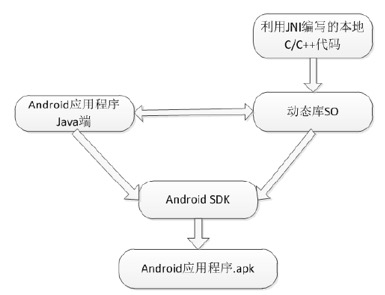
\includegraphics[width=0.8\textwidth]{figure/opencv}
%    \caption{整体框架图}
%    \label{fg:whole}
%\end{figure}

\section{手势图像预处理}

\subsection{灰度处理}

在进行视频流目标识别与跟踪时,通常第一个步骤就是对采集到的彩色图像进行灰度化\cite{黄柏林2002基于边界特征的人脸识别},这是因为黑白照片数据量小,相比彩照更易实现实时算法,另一方面黑白照片是由未处理的光线所形成的照片,因此从图像处理学角度来看,这种未经特殊滤光处理的图片所涵盖的信息更有价值。

由于在OpenCV中自带函数可以实现图像灰度化,因此在该问题处理中直接调用函数\emph{:cvCreateImage}。实现代码如下。
\begin{lstlisting}[language=C]
cvNamedWindow("image",CV_WINDOW_AUTOSIZE );//创建窗口,窗口名字为image
cvShowImage("image",img);//在刚创建的image窗口中载入图像
//创建一个与img相同大小的图像img1
IplImage *img1 = cvCreateImage(cvGetSize(img),IPL_DEPTH_8U,1);
//色彩空间转换,将源彩色图像img转化成目标灰色图像imag1
cvCvtColor(img,img1,CV_BGR2GRAY); //关键
cvNamedWindow("GrayImage",CV_WINDOW_AUTOSIZE);//创建窗口,窗口名字GrayImage
cvShowImage("GrayImage",img1);//载入转化后的图像
cvSaveImage("/lena_gray.jpg",img1,0);
\end{lstlisting}
%
%
% \begin{figure}[htb]
%    \centering
%    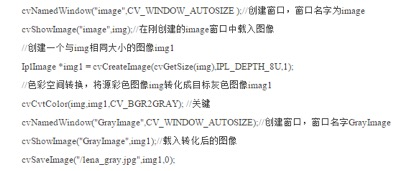
\includegraphics[width=\textwidth]{figure/hui}
%    \caption{灰度处理实现代码}
%    \label{fg:hui}
%\end{figure}

\subsection{平滑处理}

消除图像中随机噪声的技术。对平滑技术的基本要求是在消去噪声的同时不使图像轮廓或线条变得模糊不清。常用的平滑方法有中值法、局部求平均法和k 近邻平均法。局部区域大小可以是固定的,也可以是逐点随灰度值大小变化的。此外,有时应用空间频率域带通滤波方法。

对于平滑处理,在OpenCV函数库中也有相应的函数\cite{王昭威2013基于}:

\emph{CV\_BLUR\_NO\_SCALE} (简单不带尺度变换的模糊) - 对每个象素的 $param1\times param2$ 领域求和。如果邻域大小是变化的,可以事先利用函数 \emph{cvIntegral} 计算积分图像。

\emph{CV\_BLUR} (simple blur) - 对每个象素$param1\times param2$邻域 求和并做尺度变换 $1/(param1\times param2)$。

\emph{CV\_GAUSSIAN} (gaussian blur) - 对图像进行核大小为 $param1\times param2$ 的高斯卷积。

\emph{CV\_MEDIAN} (median blur) - 对图像进行核大小为$param1\times param1$ 的中值滤波 (i.e. 邻域是方的)。

\emph{CV\_BILATERAL} (双向滤波) - 应用双向 $3\times 3$ 滤波,彩色 $sigma=param1$,空间 $sigma=param2$。param1平滑操作的第一个参数。param2平滑操作的第二个参数。对于简单/非尺度变换的高斯模糊的情况,如果param2的值为零,则表示其被设定为param1。

\section{手势特征提取}

    特征提取是计算机视觉和图像处理中的一个概念。它指的是使用计算机提取图像信息,决定每个图像的点是否属于一个图像特征。特征提取的结果是把图像上的点分为不同的子集,这些子集往往属于孤立的点、连续的曲线或者连续的区域。

特征提取与选择一般分为三个步骤:特征形成、特征提取、特征选择。

特征形成  有信号获取或测量得到原始测量,之后处理后得到图像特征,这样的特征称作原始特征,如手势图像属于数字图像,它的原始测量是各点灰度值,但是这些测量不适于作为特征,还要经过计算产生一组原始特征。

     特征提取  原始特征的数量可能很大,或者说样本是处于一个多维空间中,通过映射(变换)将原始特征变换为较少的新特征,这个过程称作特征提取。映射后的特征又称作二次特征,它们是原始特征的某种组合,所以特征提取在广义上就是一种特征映射。如公式\eqref{eq:tt}所示。
\begin{equation}
    A:Y\rightarrow X
    \label{eq:tt}
\end{equation}

其中\emph{Y}是测量空间,\emph{X}是特征空间,\emph{A}称为特征映射,又称作特征提取器。

     特征选择  从原始特征中挑出一些最具有代表性和分类性最好的特征,这个过程称为特征选择,它可以起到降低特征空间维数的作用。

\subsection{Canny检测轮廓}

Canny边缘检测器利用Canny算子进行检测,是目前最精确的检测器,并且已经被大量运用于程序中。从目前看来,canny边缘检测在做图像轮廓提取 方面是最优秀的边缘检测算法。

canny边缘检测采用双阈值值法,高阈值用来检测图像中重要的、显著的线条、轮廓等,而低阈值用来保证不丢失细节部分,低阈值检测出来的边缘更丰富,但是很多边缘并不是我们关心的。最后采用一种查找算法,将低阈值中与高阈值的边缘有重叠的线条保留,其他的线条都删除。

函数如下:
\begin{lstlisting}[language=C]
int main() 
{ 
    Mat I=imread("../cat.png"); 
    cvtColor(I,I,CV_BGR2GRAY); 
                                                 
    Mat contours; 
    Canny(I,contours,125,350); 
    threshold(contours,contours,128,255,THRESH_BINARY); 
    namedWindow("Canny"); 
    imshow("Canny",contours); 
    waitKey(); 
    return 0; 
} 
\end{lstlisting}
效果如图\ref{fg:Canny}所示。
\begin{figure}[htb]
    \centering
    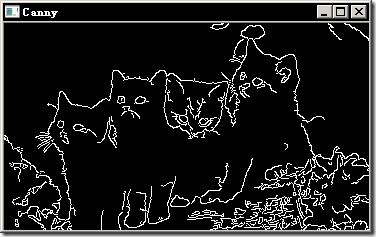
\includegraphics[width=0.8\textwidth ]{figure/cat}
    \caption{Canny轮廓检测效果图}
    \label{fg:Canny}
\end{figure}


\subsection{直线检测}

直线在图像中出现的频率非常之高,而直线作为图像的特征对于基本内容的图像分析有着很重要的作用,我们通常通过OpenCV中的hough变换来检测图像中的线条。

首先展示最基本的Hough变换函数HoughLines,它的原型如下所示。
\begin{lstlisting}
void HoughLinesP(InputArray image, OutputArray lines, double rho, double theta,int threshold, double minLineLength=0, double maxLineGap=0 ); 
\end{lstlisting}
%\begin{figure}[htb]
%    \centering
%    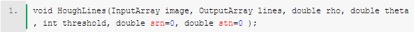
\includegraphics[width=\textwidth]{figure/code}
%    \caption{HoughLines原型}
%    \label{fg:yuan}
%\end{figure}

 

    它的输入是一个二值的轮廓图像,往往是边缘检测得到的结果图像;它的输出是一个包含多个\emph{Vec2f}点的数组,数组中的每个元素是一个二元浮点数据对\emph{<rou,theta>}而言,\emph{rou}代表直线离坐标原点的距离,\emph{theta}代表角度。第3和第4个参数代表步长,因为\emph{Hough}变换实际上是一个穷举的算法,\emph{rho}表示距离的步长,\emph{theta}代表角度的步长。第5个参数是一个阈值设置直接的最低投票个数,知道\emph{Hough}原理的,这个参数应该很容易理解。

   从这个函数的输出结果我们可以看出,得到的直线并没有指定在图像中的开始点与结束点,需要我们自己去计算,如果我们想把直接显示在图像中就会比较麻烦,而且 会有很多角度接近的直线,其实它们是重复的,为了解决上面这些问题,\emph{OpenCV}又提供了一个函数\emph{HoughLinesP()}。它的输出是一个 \emph{Vector of Vec4i}。\emph{Vector}每一个元素代表一条直线,是由一个4元浮点数组构成,前两个点一组,后两个点一组,代表了在图像中直线的起始和结束点。

\subsection{轮廓的提取与描述}

在目标识别中,首先要把感兴趣的目标提取出来,而一般常见的步骤都是通过颜色或纹理提取出目标的前景图(一幅黑白图像,目标以白色显示在图像中),接下来要对前景图进行分析进一步地把目标提取出来,而这里常常用到的就是提取目标的轮廓。

OpenCV 里提取目标轮廓的函数是\emph{findContours},它的输入图像是一幅二值图像,输出的是每一个连通区域的轮廓点的集 合:\emph{vector<vector<Point>>}。外层\emph{vector}的\emph{size}代表了图像中轮廓的个数,里面\emph{vector}的\emph{size}代表了轮廓上点的个数。

提取到轮廓后,最重要的就是如何把这些轮廓转换为可以利用的特征,也就是涉及到轮廓的描述问题,这时就有多种方法可以选择,比如矢量化为多边形、矩形、椭圆等。OpenCV里提供了一些相应函数,在这里就不详细介绍了。 
\section{照相机线程冲突解决方案}
由于Android系统原因,Camera为一个非共享资源,即同一时间只能由一个线程使用。而我们的拍照手势识别算法的目的就是用手势控制相机,故必然要有相机的预览。这时就存在着一个难点:如何让预览和OpenCV的VideoCapture同时获得图像。

传统上,面对此问题有两种解决方案:
\begin{enumerate}
    \item 利用两个线程分时占用相机,交替获得控制权。
    \item 利用VideoCapture从相机获得图片,再传入前端View渲染。
\end{enumerate}
这两种方法固然可以解决,但是方法1,由于交替切换控制权,存在大量延时。而方法2除去编码复杂,更是OpenCV的VideoCapture采集的祯尺寸一般是线程初始化是就预设好的,而为了处理速度,一般都设为较小尺寸,但是如果直接在前端渲染,则就会过于模糊。因此,传统上并没有解决此问题的好方法。

本算法中,我们采用类似于方法2的方法,但是我们采用了间隔采集和预设尺寸两种方法兼顾了速度与相片质量。
\begin{enumerate}
    \item 间隔采集:顾名思义,就是每隔一定的间隔才采集一帧画面,我们采取每40ms采集一次,即25FPS,保证了预览的流畅,同时降低了运算复杂度,保证了速度。
    \item 预设尺寸:前文说到,VideoCapture是在线程初始化时预设好尺寸的,因此我们就在一开始预设了较大的尺寸,而由于间隔采集,大尺寸并不会造成太大的处理压力,我们先将大尺寸彩色图片传至前端渲染,再将其缩小灰度化后传入后端计算。从而保证了预览质量和相片质量。
\end{enumerate}



\chapter{算法设计与实现}
本章主要介绍了本算法选取的手势,手势识别的具体过程,及整个算法的封装结构。
\section{手势选取}
考虑到本算法为手势拍照设计的专用算法,故手势不需太多。为了保证识别性能,我们采用动态手势来作为算法识别的手势,即上划,下划,左划,右划四个基本手势。
\section{识别过程}

\section{算法封装结构}

\ifx\allfiles\undefined
%\bibliographystyle{unsrt}
\bibliography{main}
\end{document}
\fi